\section{Logical view}

Som beskrevet i view beskrivelserne på forrige side består logical viewet af designoverview-, sekvens-, statemachines samt klassediagrammer. Til at udforme diagrammerne anvendes applikationsmodellen.

\subsection{Applikationsmodel}
Med applikationsmodellen tages der udgangspunkt i use cases beskrevet i kravspecifikationen og domain modellen, se figur \ref{fig:domain_model}.
  
Ud fra domain modellen identificeres de overordnede klasser der skal bruges til de forskellige iterationer. Når de overordnede klasser er identificeret beskrives hvordan de kommunikerer via desginoverview og sekvensdiagrammer. Herefter laves statemachines med de fundne klasser og til sidst udarbejdes klassediagrammer.


\subsection{Iteration \#1}
I iteration 1 arbejdes der med blokke som dækker over systemets mest grundlæggende funktionalitet. Batteri,
ESC’er, motorer og sensorer tilsluttes dronen. Desuden gøres dronen i stand til oprette forbindelse til webapplikation via 3G-shield’et. Hvordan systemet er tiltænkt at bruges beskrives i user story nedenfor:

\subsubsection*{User story}
Bruger tænder dronen ved at tilslutte batteri. Main controller samt 3G/GPS module initialiseres og nuværende GPS position opdateres. Herefter oprettes forbindelse mellem drone og webapplikation, og information om dronen er online samt information om dronens nuværende GPS position sendes til webapplikation. Fra webapplikationen er det muligt for bruger løbende at observere hvorvidt dronen er online og på hvilken GPS position dronen sidst har befundet sig.

%kommentar
\begin{figure}[H]
	\centering
	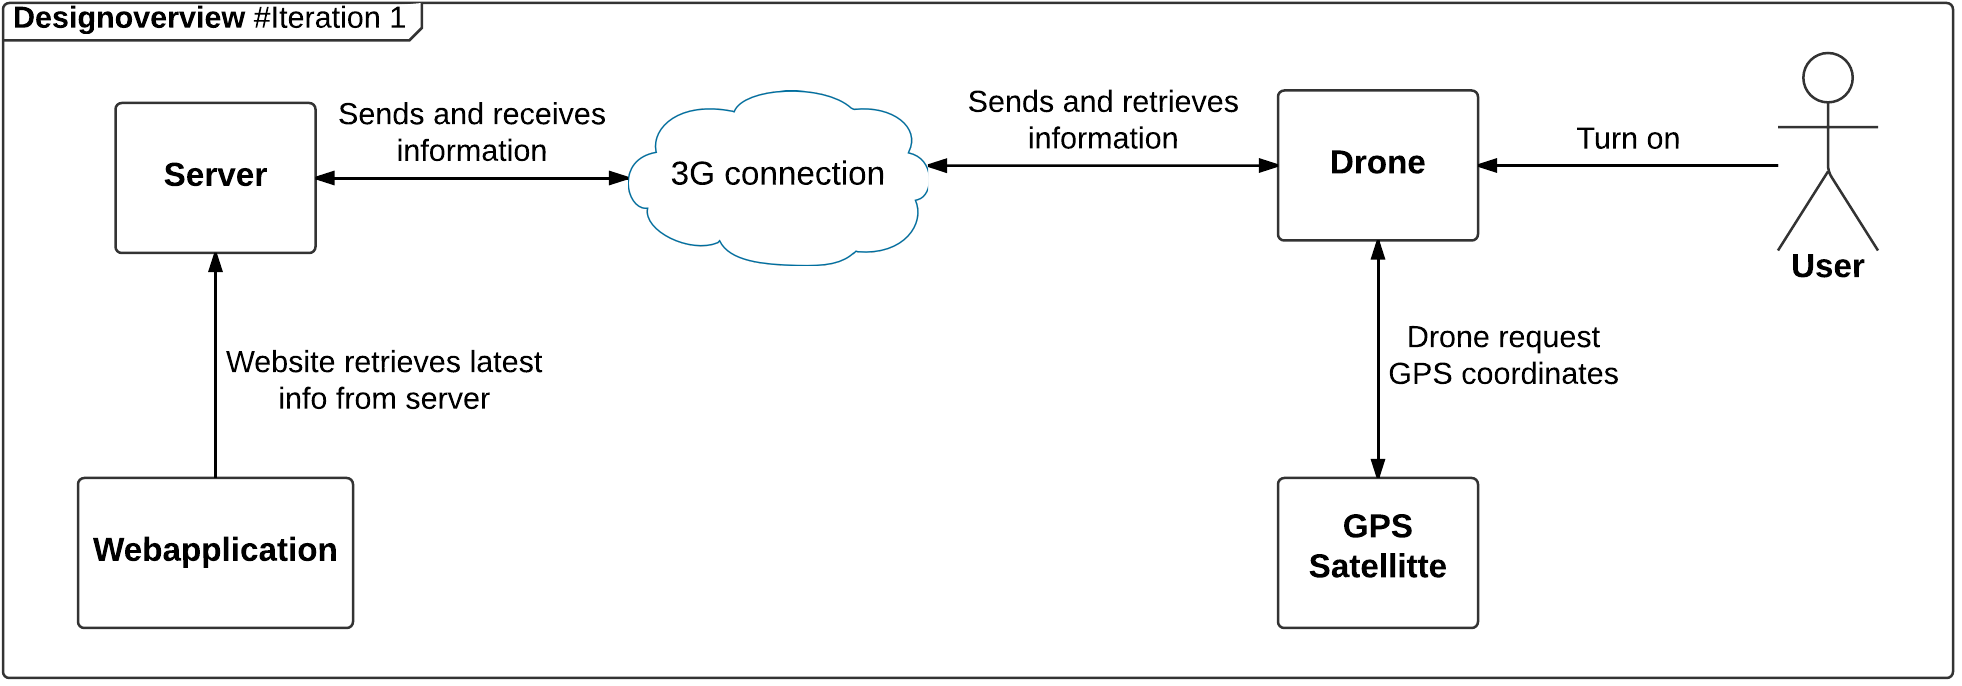
\includegraphics[width=1\textwidth]{Billeder/design_overview/design_overview_iteration1.png}
	\vspace{-.5cm}
	\caption{Design overview \#iteration 1}
	\label{fig:design_overview_UC1}
\end{figure}


\newpage
\subsubsection*{Sekvens diagram}
På sekvensdiagrammet på figur \ref{fig:Sekvens_diagram_iteration1}, vises hvilke klasser der indgår og bruges i første iteration. Af sekvensdiagrammet fremgår det, at sekvensen først startes når bruger tilslutter batteri og tænder dronen. Når der er tilkoblet forsyning initialiseres main controller samt 3G/GPS og nuværende GPS position  (longitude og latitude) opdateres. Dronens nuværende GPS position opdateres når dronen sender PUT requests til webapplikation. PUT requests bruges dels til at fortælle webapplikationen at dronen er online og dels til at give webapplikation information om dronens nuværende position. 


%kommentar
\begin{figure}[H]
	\centering
	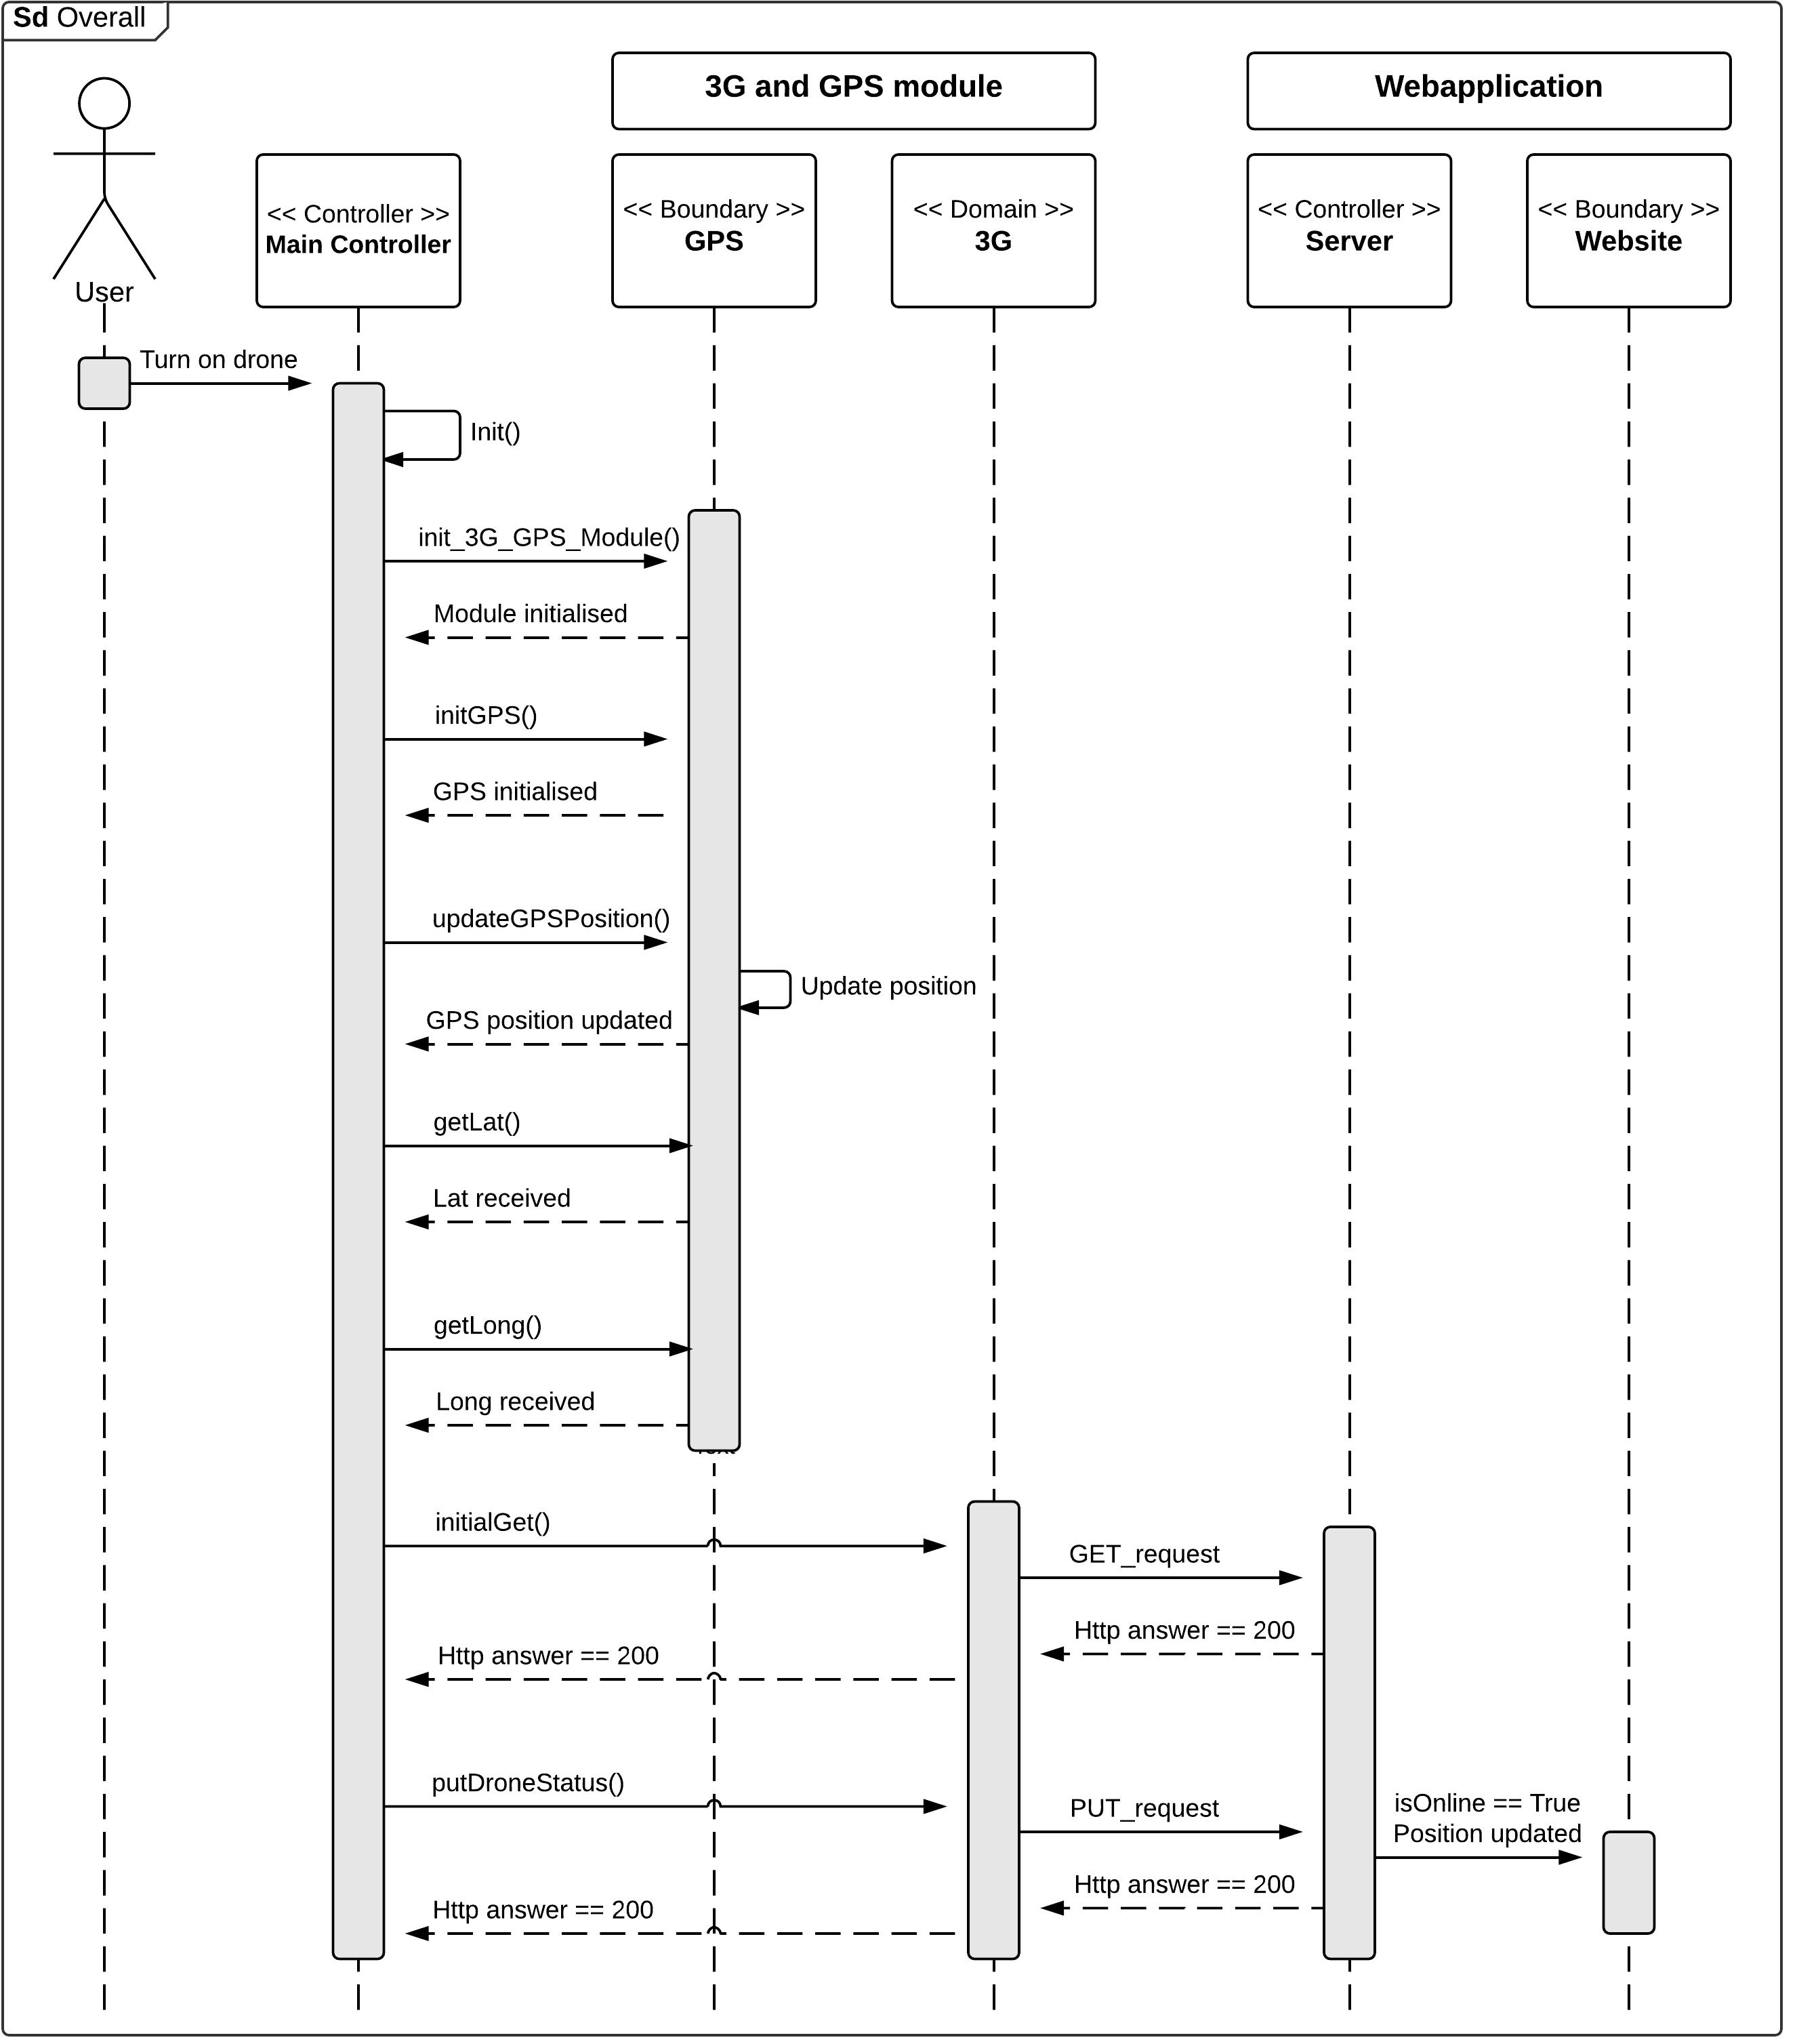
\includegraphics[width=0.93\textwidth]{Billeder/sekvens/sekvens_iteration1}
	\caption{Sekvens diagram \#iteration 1}
	\label{fig:Sekvens_diagram_iteration1}
\end{figure}

\newpage
\subsubsection*{State machine diagram}
\vspace{-0.1cm}
I state machine diagrammet på figur \ref{fig:Statemachine_iteration1}, vises de forskellige states der eksisterer i iteration 1 og hvordan flowet imellem dem ser ud. Der eksisterer givet vis kun 2 states i iteration 1, men state machinen er medtaget fordi den på nem og overskuelig vis illustrerer systemflowet.
%kommentar
\begin{figure}[H]
	\centering
	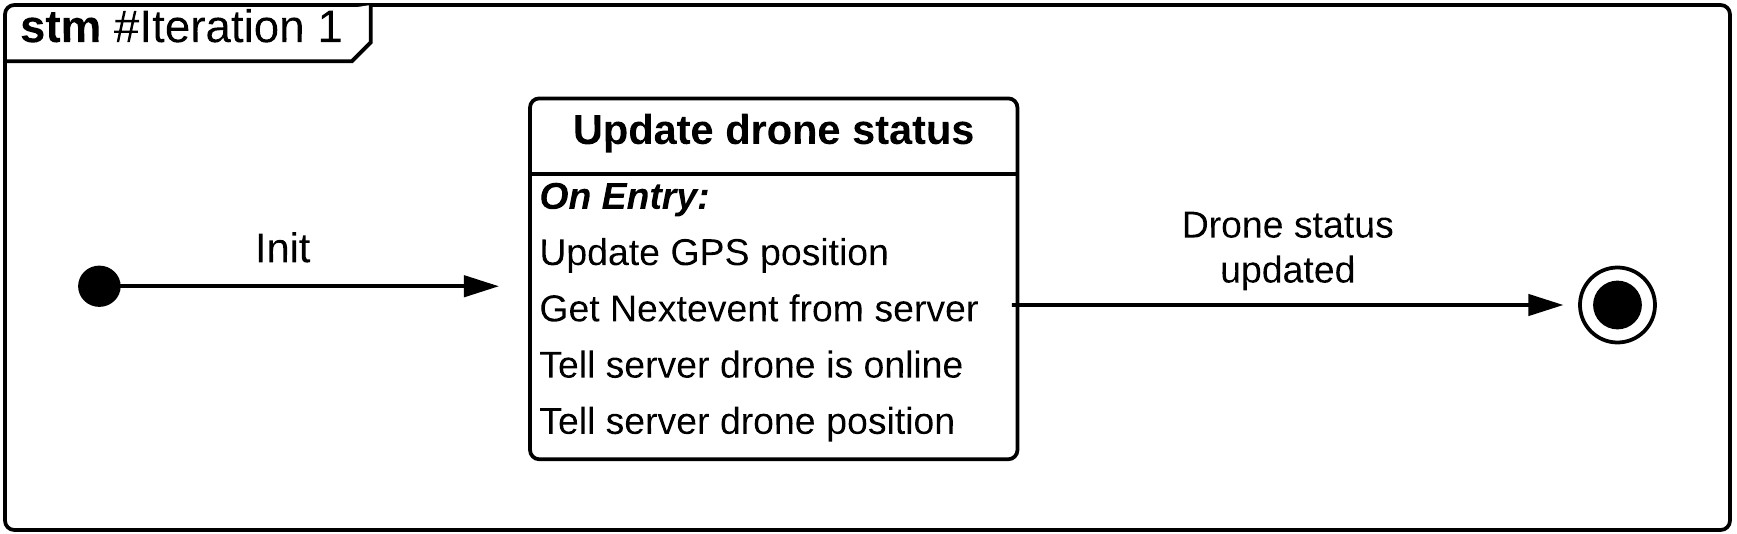
\includegraphics[width=1\textwidth]{Billeder/statemachine/State_iteration1.png}
	\vspace{-0.5cm}
	\caption{Statemachine \#iteration 1}
	\label{fig:Statemachine_iteration1}
\end{figure}

\subsubsection*{Klasse diagram}
\vspace{-0.1cm}
Figur \ref{fig:classDiagram_iteration1} vises et klassediagram tilhørende iteration 1. Klassediagrammet viser iterationens vigtigste klasser, samt deres tilhørende metoder og attributter. På den følgende side forefindes en kort beskrivelse klasserne og deres metoder.
%kommentar
\begin{figure}[H]
	\centering
	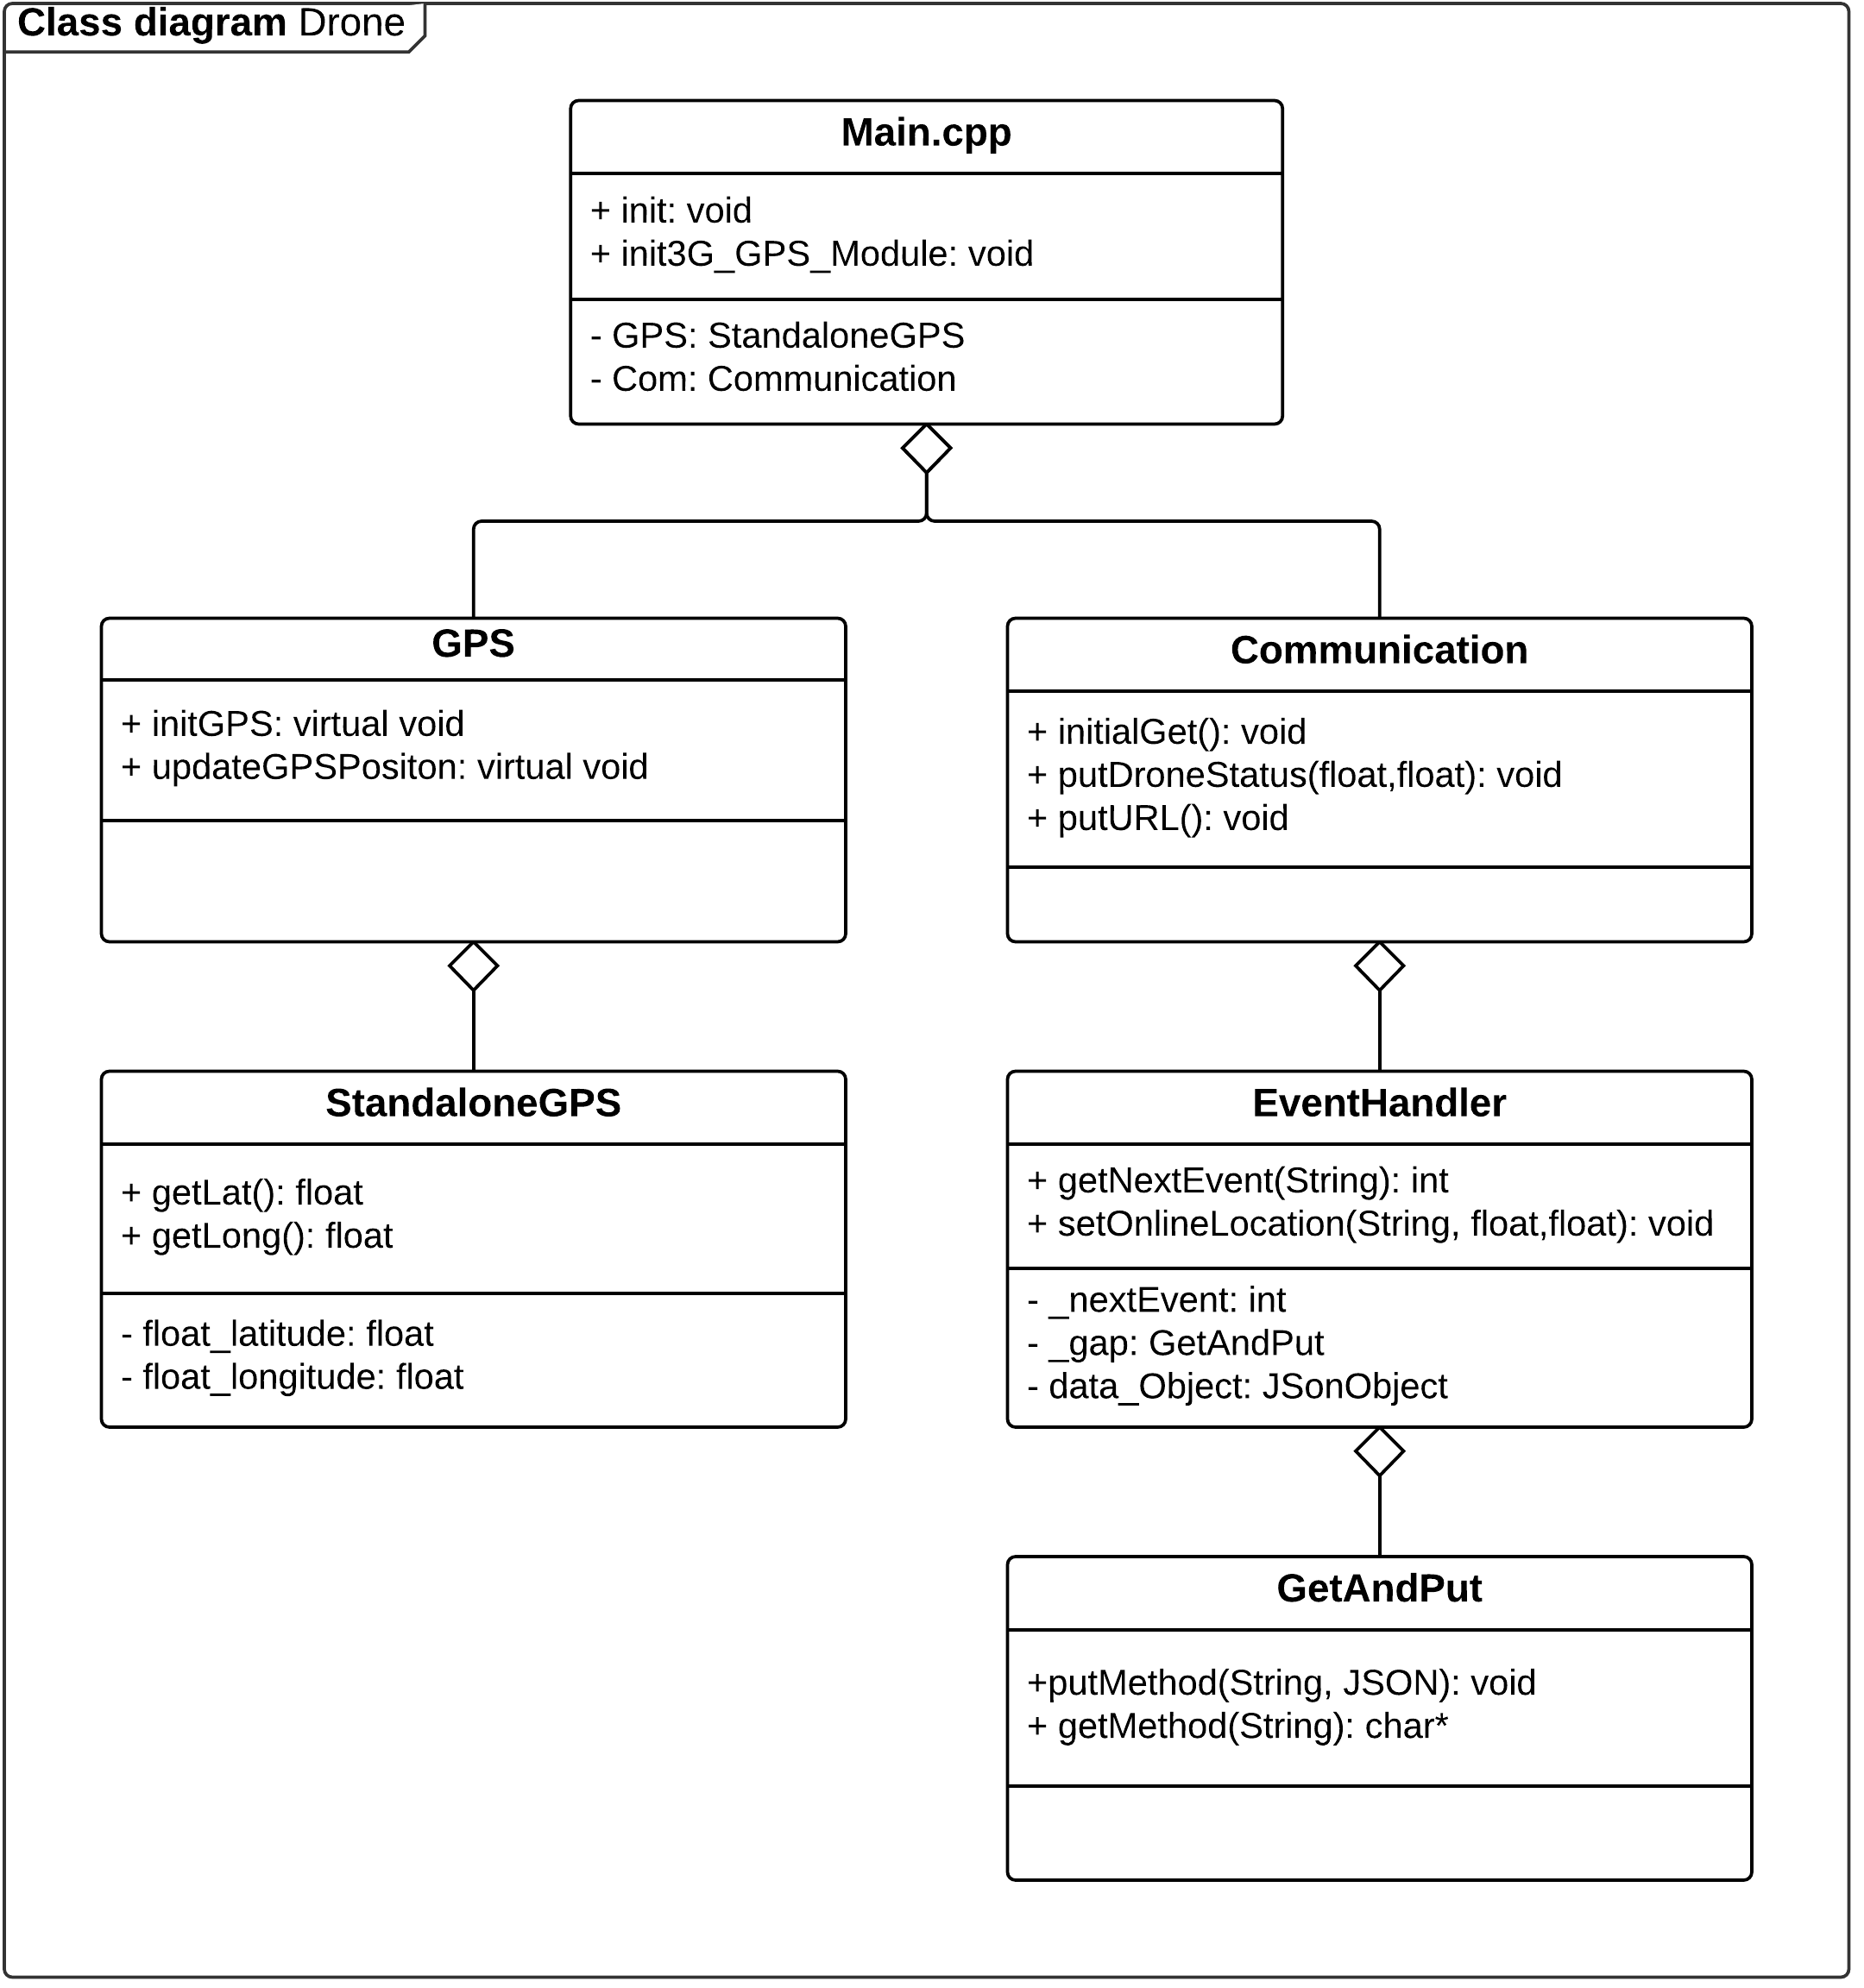
\includegraphics[width=1\textwidth]{Billeder/klasse_diagrammer/classdiagram_iteration1.png}
	\vspace{-0.5cm}
	\caption{Klassediagram \#iteration 1}
	\label{fig:classDiagram_iteration1}
\end{figure}

\newpage

\textbf{Main.cpp} \\
Main.cpp filen bruges til at sætte arduino board korrekt op, bla. sættes baudrate på de forskellige serielle forbindelser. Desuden bruges Main.cpp til at kalde og eksekverer forskellige klasse, objekter og funktioner.

\textbf{GPS} \\
GPS klassen fungerer som en virtuel klasse, og sikre som minimum implementering af init og updateGPSPosition uanset hvilken GPS der bruges. Klassen er lavet fordi der i udgangspunkt var mulighed for at bruge 3 forskellige slags GPS med 3G/GPS shieldet. 

\textbf{StandaloneGPS}\\
Denne klasse er ansvarlig for al kommunikation med GPS'en når standalone mode er valgt. 

\textbf{Module\_3G} \\
Module\_3G er ansvarlig for alt kommunikation mellem drone og server. I klassen bruges to forskellige slags http request. Når der ønskes at trække information fra sever til drone gøres der brug af GET request mens der gøres brug af PUT request når dronen ønsker at informere server om ny lokation.




\newpage

\subsection{Iteration \#2}
I iteration 2 er formålet dels at få styr på websitet og dels at få styr på den autonome flyvning. Bruger skal kunne oprette flyveopsætninger og gøre dem tilgængelig for dronen, hvilket kræver der er styr på kommunikationen mellem webserver og drone. Ydermere skal dronen kunne finde egen GPS position, flyvehøjde og orientering. Ud fra viden om egen position, flyvehøjde og orientering skal dronen flyve til de lokationer som er fastsat i flyveopsætningen. 
Hvordan systemet er tiltænkt at bruges beskrives i user story nedenfor:

\subsubsection*{User story}
Bruger logger på webapplikationen med sit brugernavn og password. Når der er logget korrekt ind vises bruger sin eller sine droner på en liste. Ved at trykke på en drone vises bruger information om den pågældende drone. Informationen beståer af waypoints, om der skal tages billeder ved de forskellige waypoints samt indstilling af flyvehøjde. Ønsker bruger at oprette en ny flyveopsætning............

Når en drone er tændt og færdig initialiseret fortæller den server webserveren om sin nuværende position og kontrollerer om en ny flyveopsætning er tilgængelig. Er der en ny flyveopsætning tilgængelig hentes den og dronen påbegynder flyvning.

%kommentar
\begin{figure}[H]
	\centering
	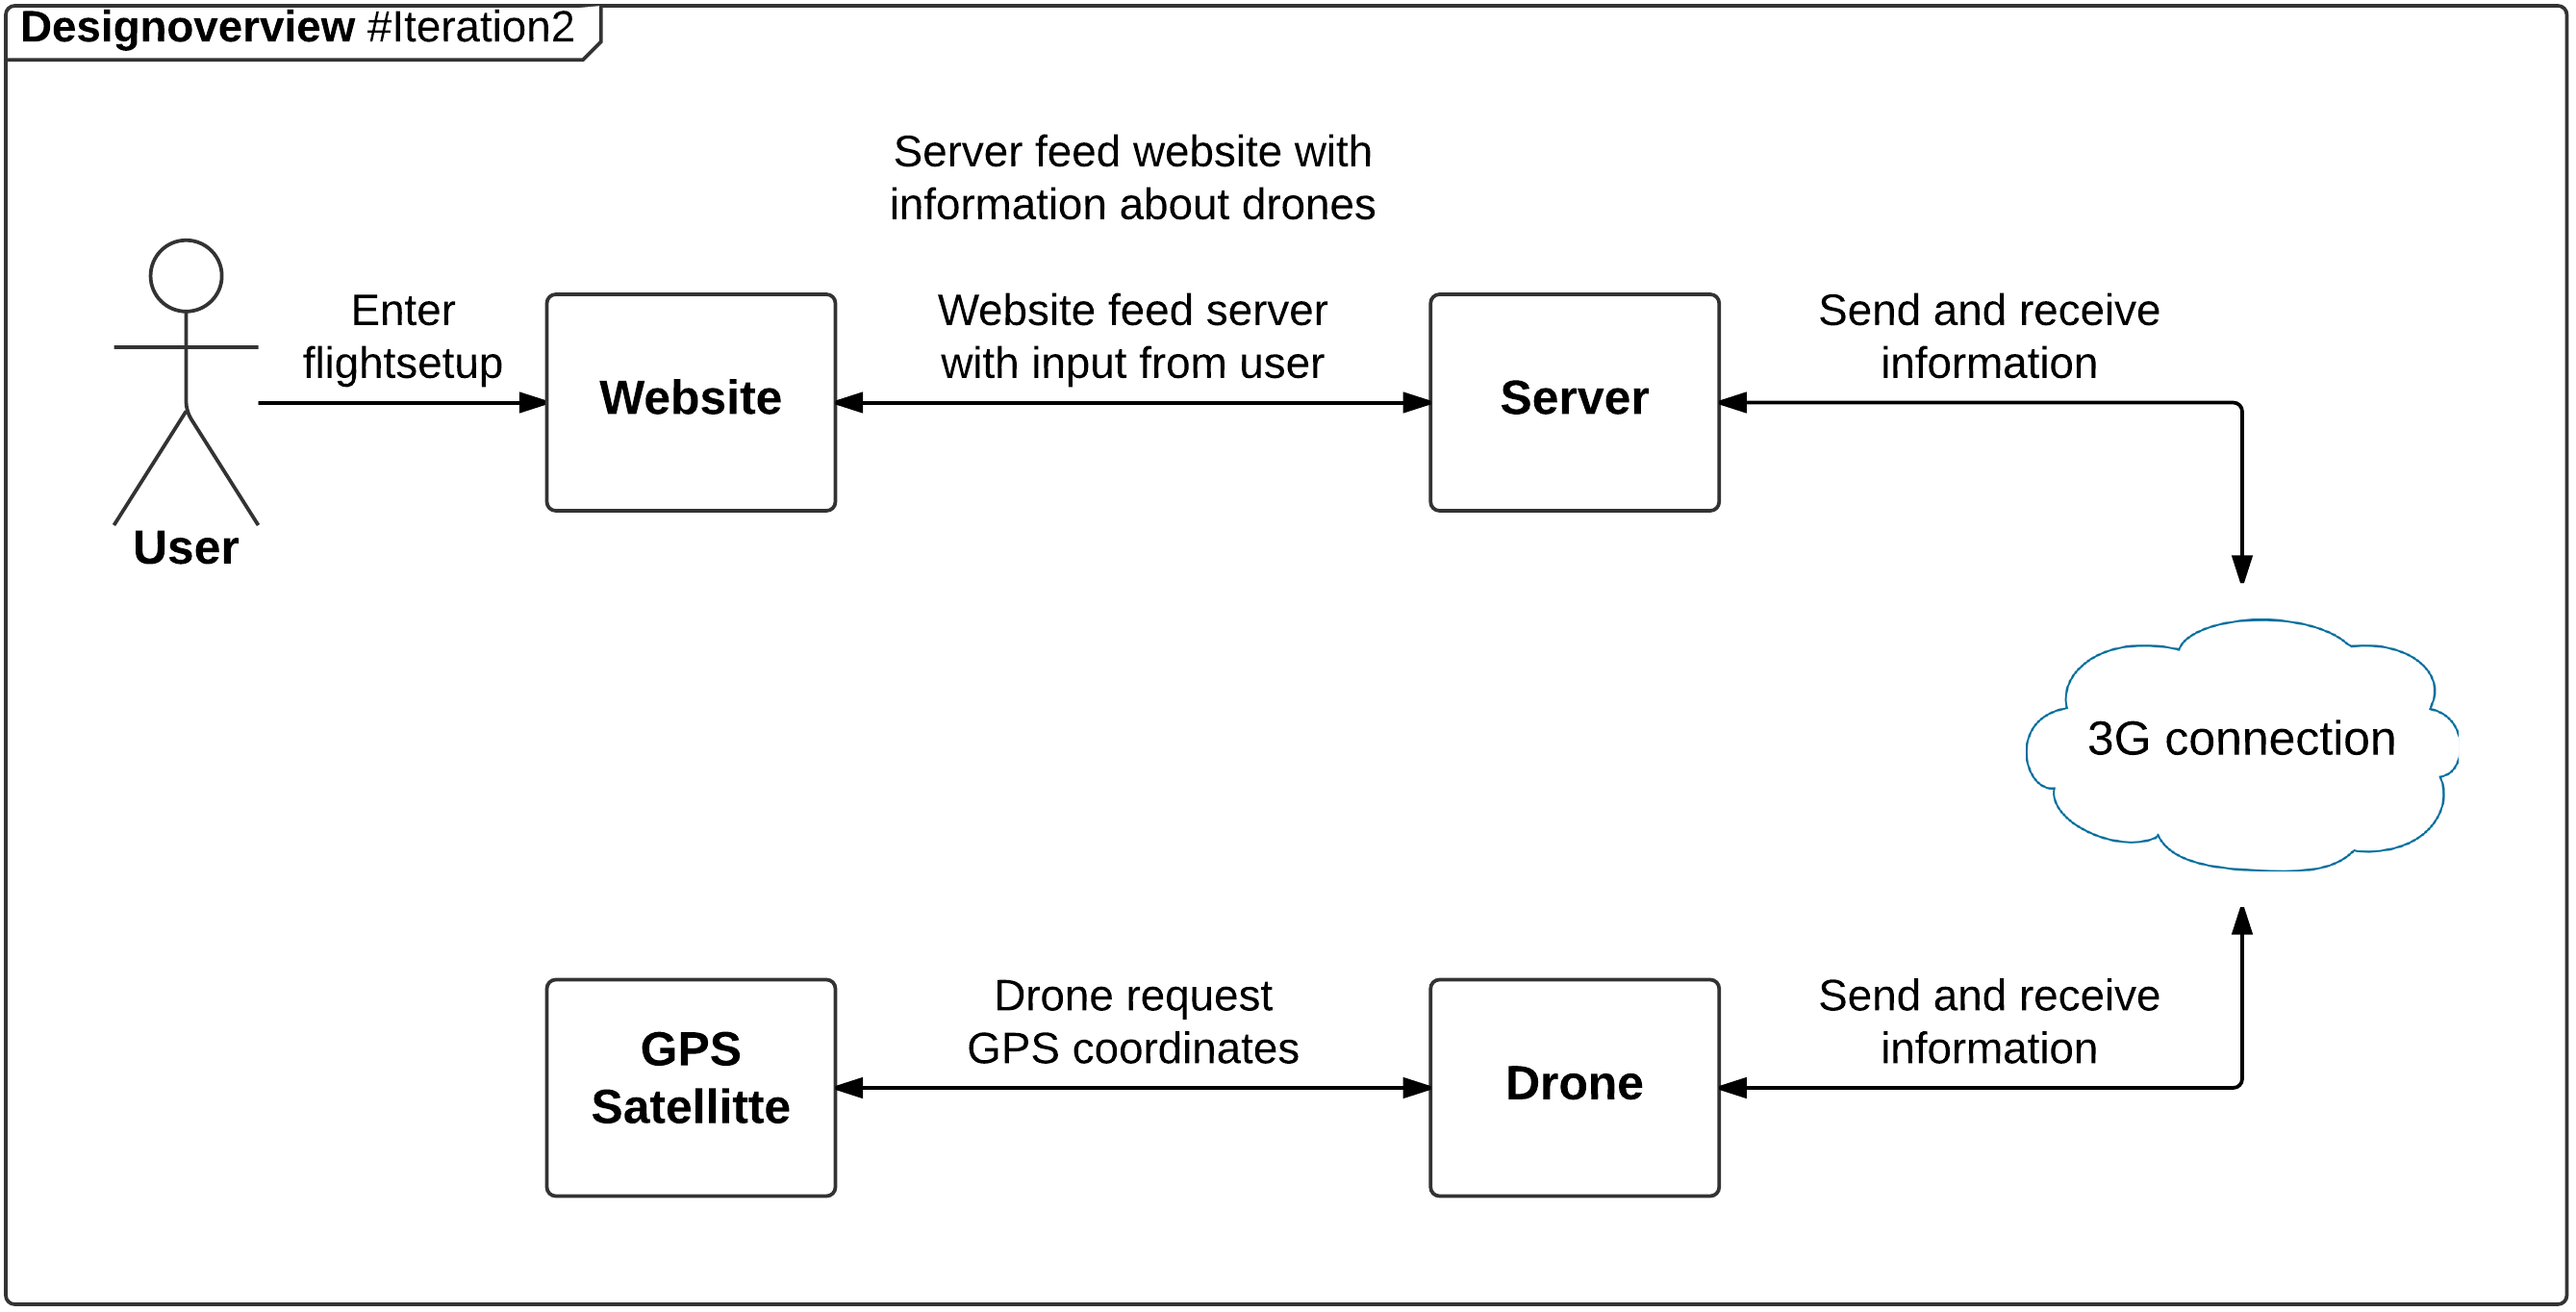
\includegraphics[width=1\textwidth]{Billeder/design_overview/design_overview_iteration2.png}
	\vspace{-.5cm}
	\caption{Designoverview \#iteration 2}
	\label{fig:design_overview_UC1}
\end{figure}



\newpage

\subsubsection*{Sekvens diagram}

Til iteration 2 er systemsekvensen beskrevet med 3 mindre sekvensdiagrammer i stedet for 1 stort. 
Denne fremstilling gør det muligt at repræsentere systemets funktionalitet på mere overskuelig vis, hvilket burde gøre indirekte øger forståelsen af diagrammerne. Hvert af de 3 sekvensdiagrammet bruges til at fortælle hvordan en delmængde af systemet fungerer.

Af figur \ref{fig:Sekvens_diagram_iteration2_1} fremgår det hvordan bruger opretter en ny flyveopsætning. Det vises desuden hvilke interaktioner der foretages mellem bruger og website, samt hvordan server løbende indgår og benyttes i sekvensen. 

%kommentar
\begin{figure}[H]
	\centering
	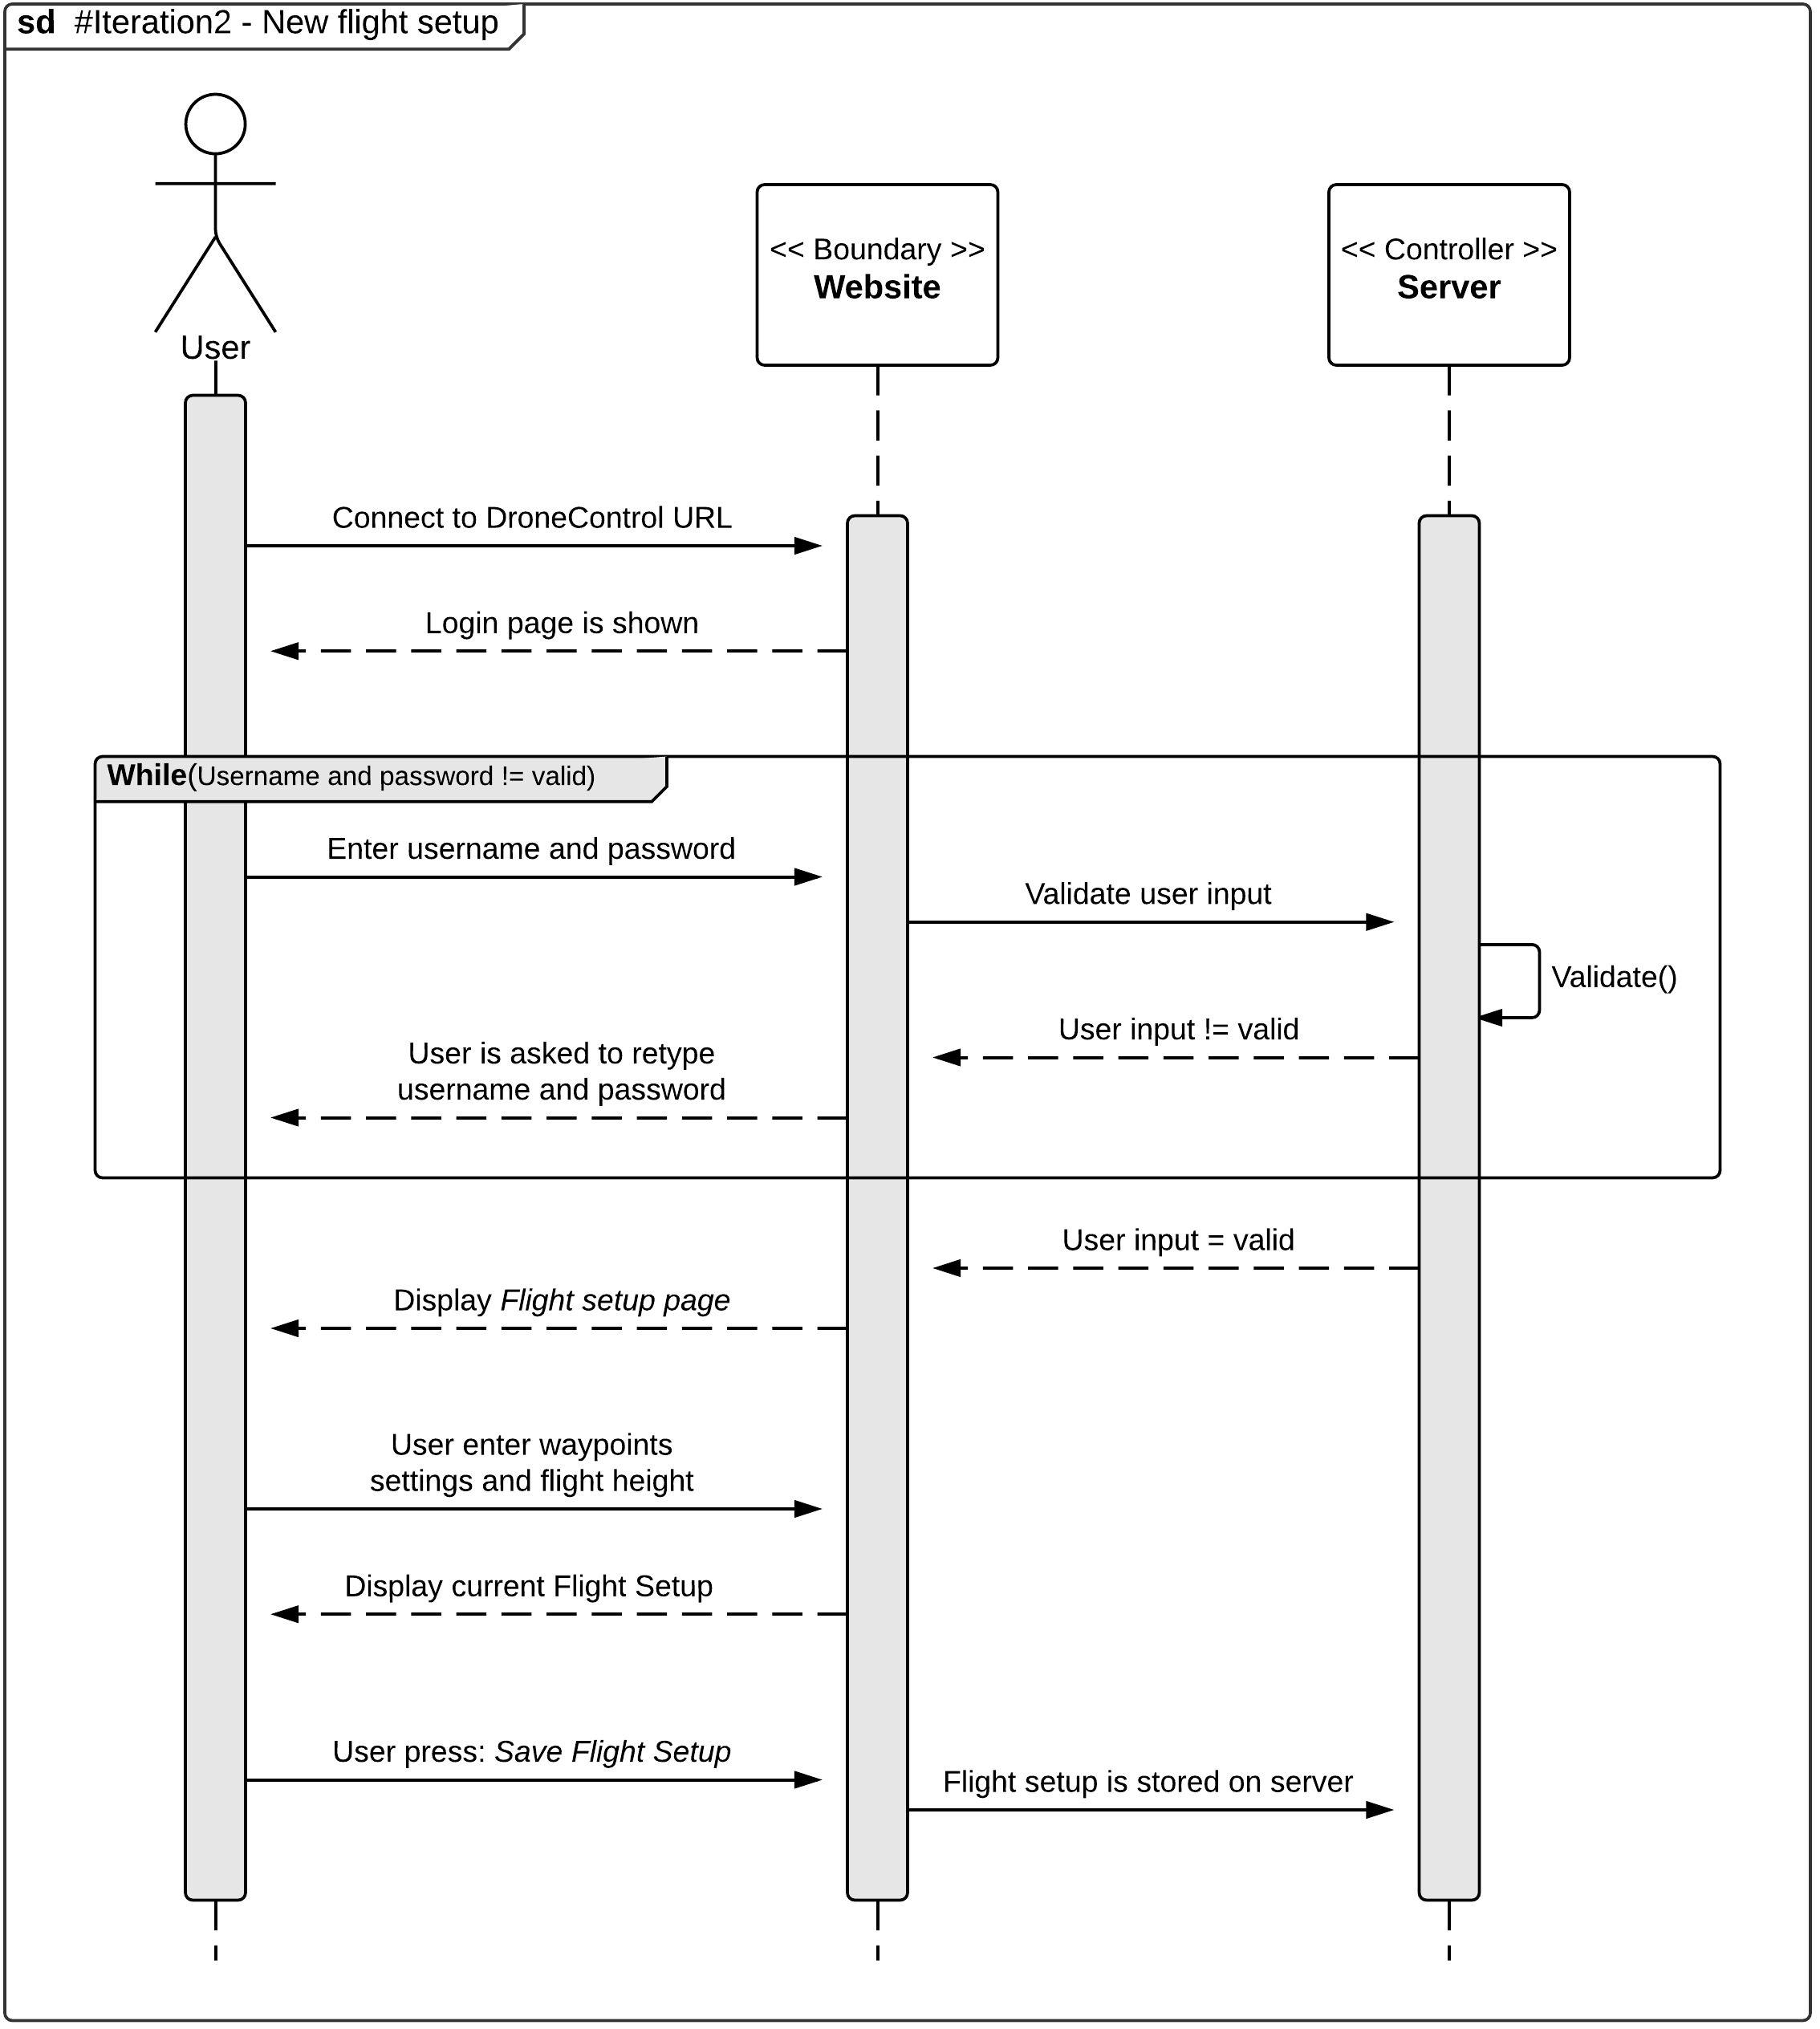
\includegraphics[width=1\textwidth]{Billeder/sekvens/sekvens_iteration2_1}
	\caption{Sekvensdiagram \#iteration 2}
	\label{fig:Sekvens_diagram_iteration2_1}
\end{figure}


\newpage

På figur \ref{fig:Sekvens_diagram_iteration2_2} fremgår det hvordan dronens main controller via 3G-shieldet kommunikerer med serveren for at kontrollere om der er en ny flyveopsætning tilgængelig. Det vises også hvilke beskeder der flyder frem og tilbage mellem main controller og server. Desuden vises det at dronen først henter ny flyveomsætning, når serveren har bekræftet, at der er en flyveopsætning tilgængelig.   

%kommentar
\begin{figure}[H]
	\centering
	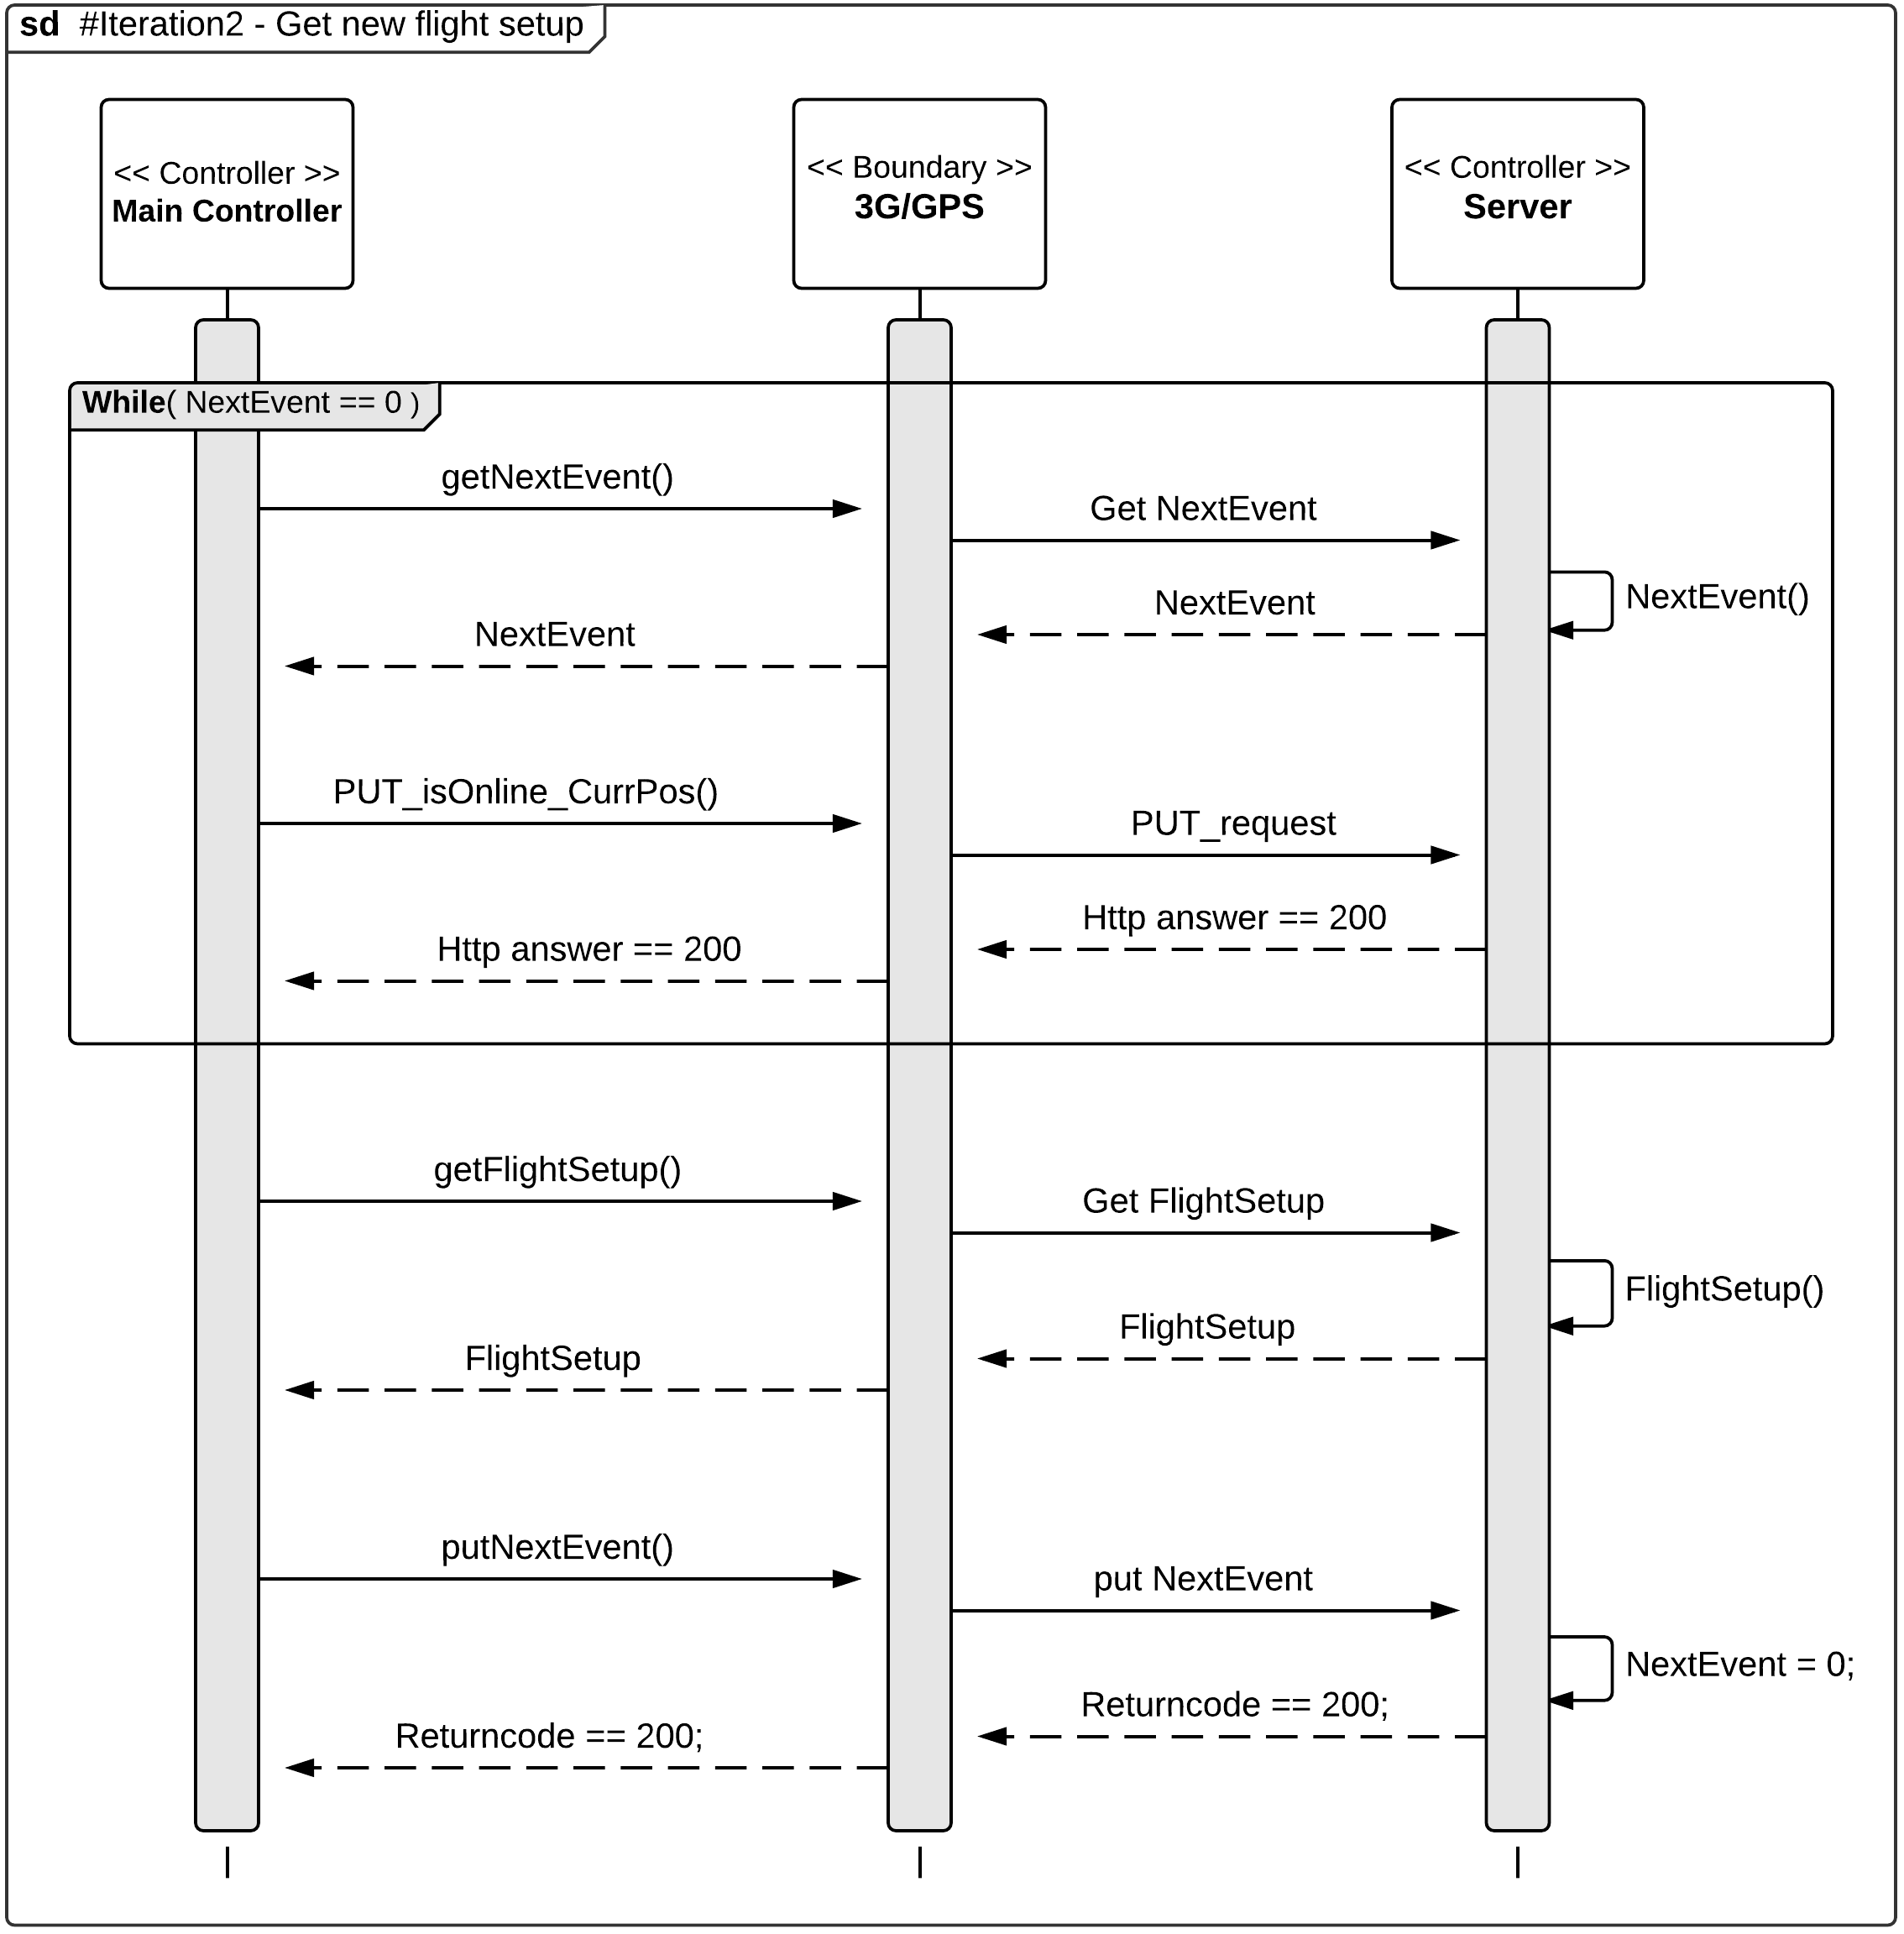
\includegraphics[width=1\textwidth]{Billeder/sekvens/sekvens_iteration2_2}
	\caption{Sekvensdiagram \#iteration 2}
	\label{fig:Sekvens_diagram_iteration2_2}
\end{figure}

\newpage

Af figur \ref{fig:Sekvens_diagram_iteration2_3} fremgår det hvordan dronen opererer når den flyver autonomt mod en givet GPS position. Main controlleren indsamler kompas data fra flight control boardet, latitude og longitude fra 3G/GPS modulet og flyvehøjde fra ultralyds sensoren. Den indhentede data processeres og bruges til at korrigerer de nuværende flyveindstillinger.
Som det fremgår af while loopet fortsætter flyvningen indtil dronen er 15 meter fra den GPS bruger valgte i flyveopsætningen. 


%kommentar
\begin{figure}[H]
	\centering
	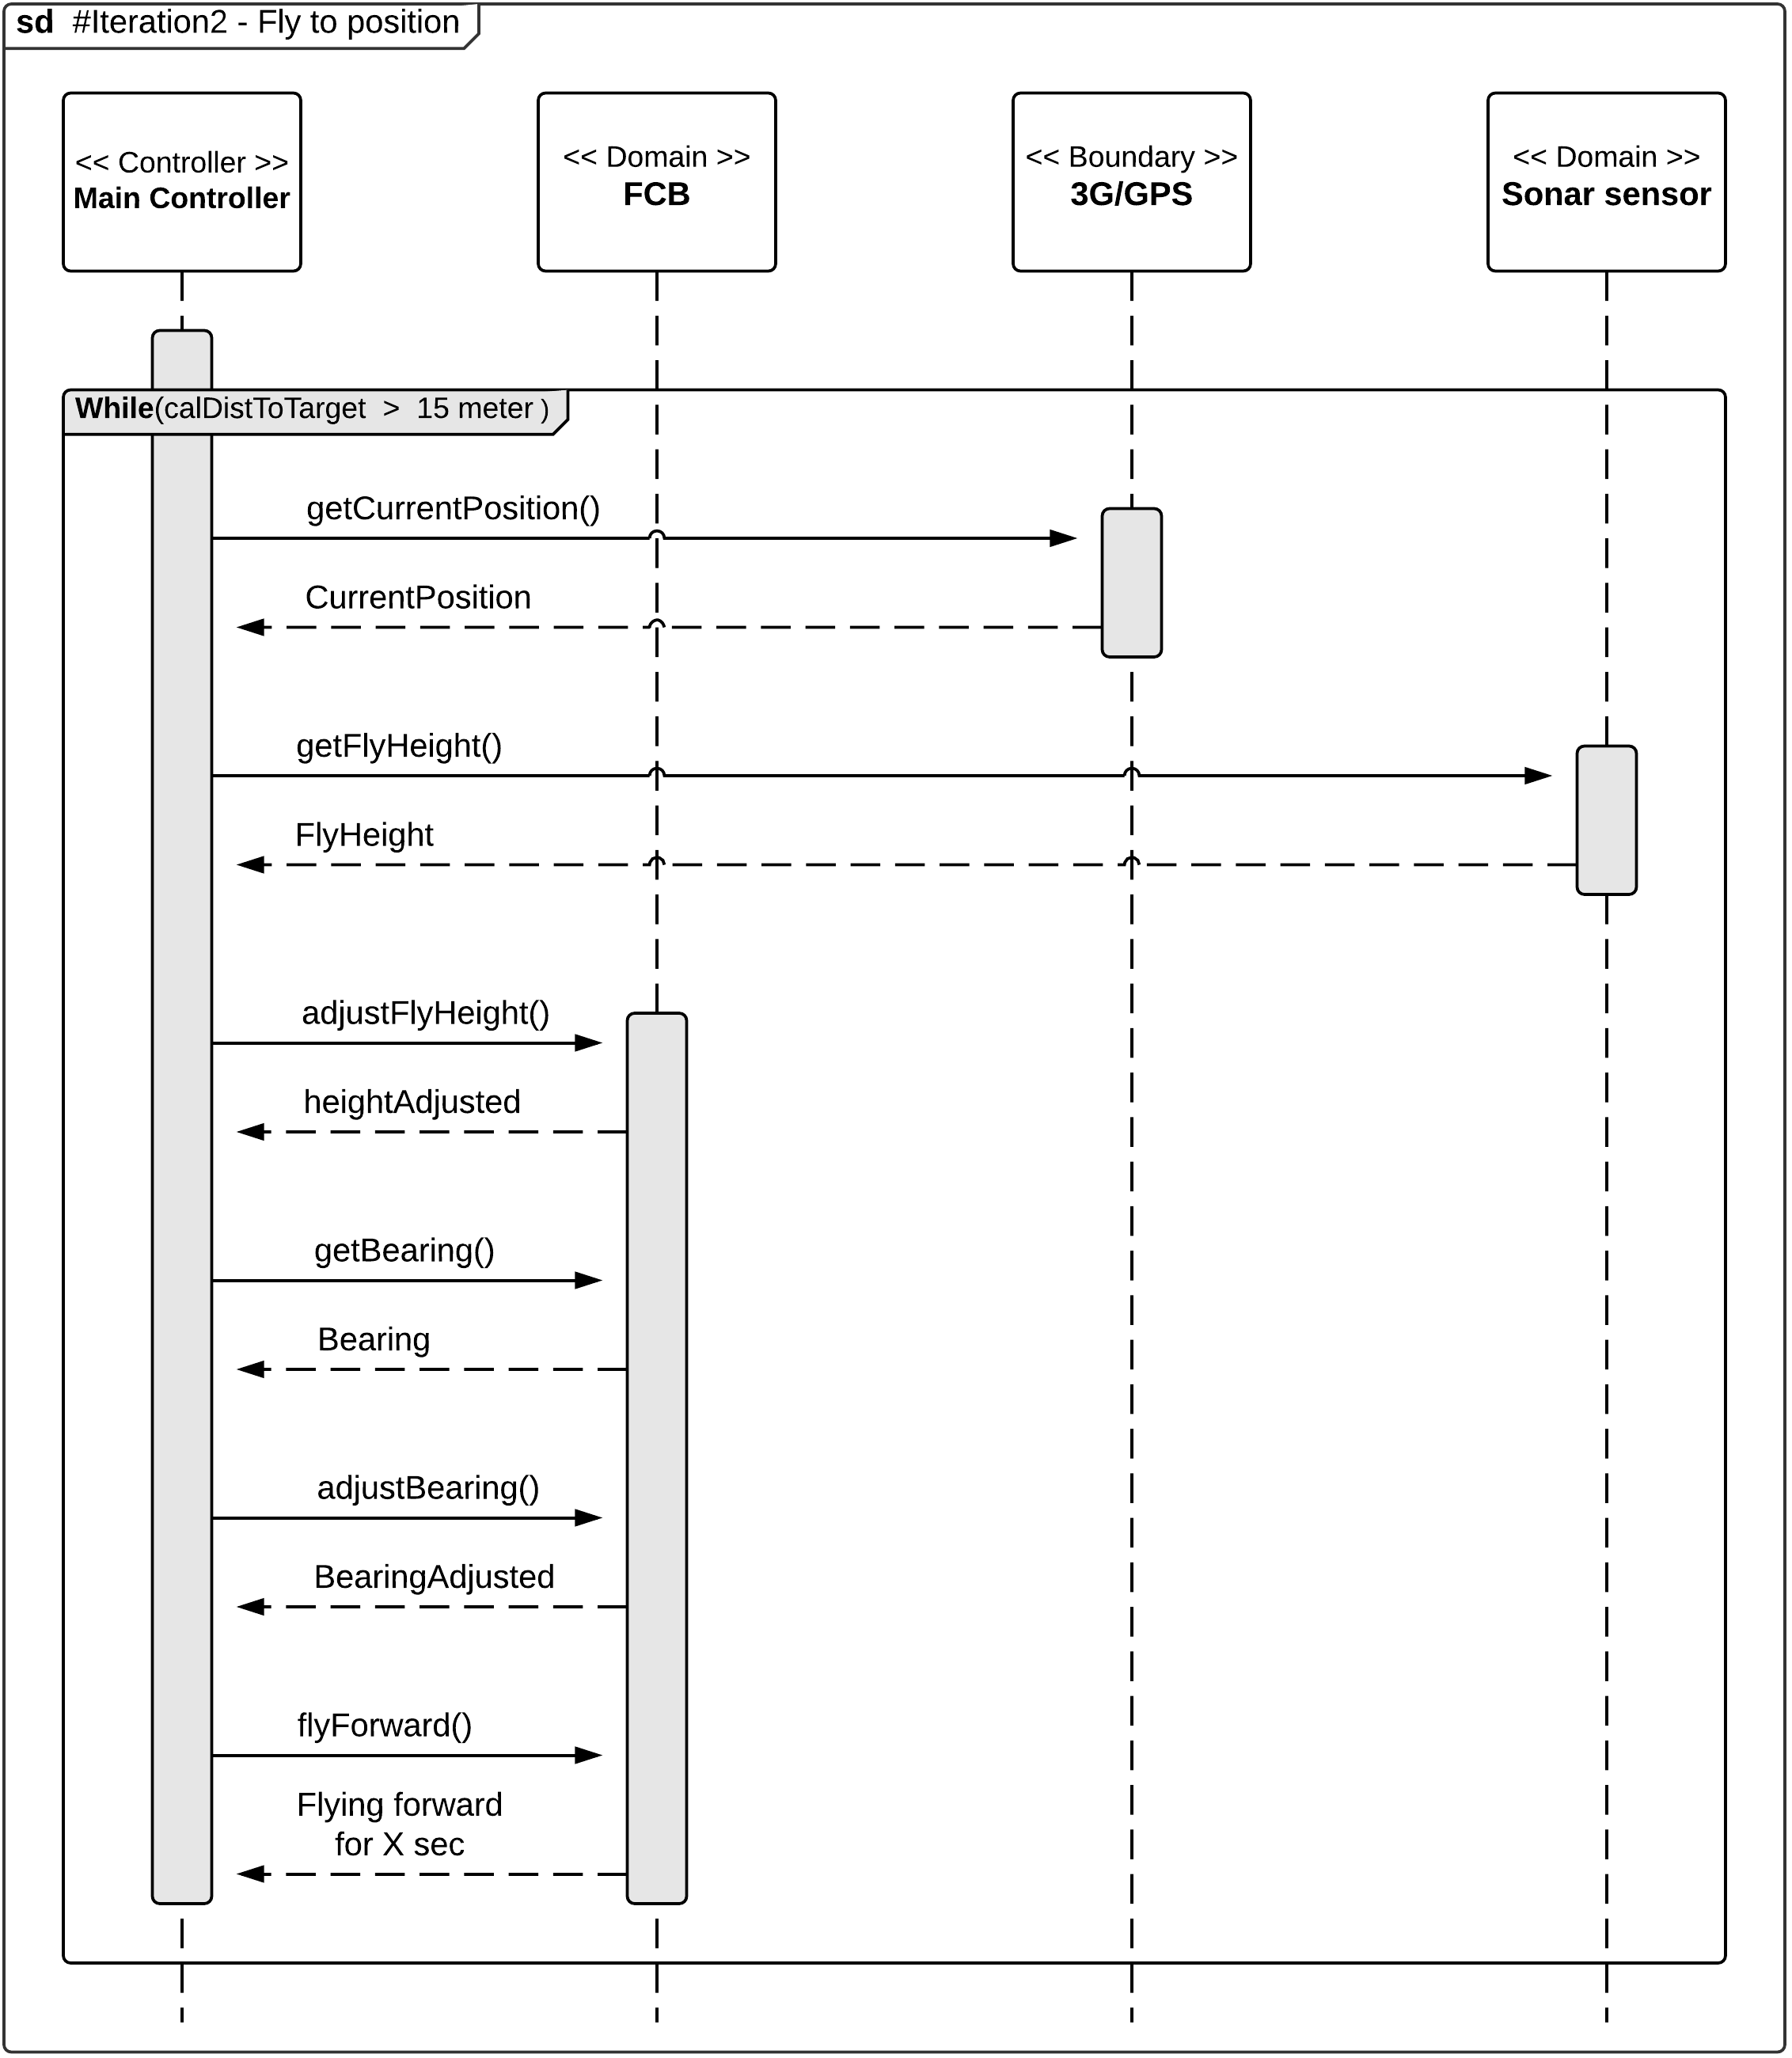
\includegraphics[width=1\textwidth]{Billeder/sekvens/sekvens_iteration2_3}
	\caption{Sekvensdiagram \#iteration 2}
	\label{fig:Sekvens_diagram_iteration2_3}
\end{figure}